\chapter{Results}

\todo[inline]{Analysis of results}

\section{Semi-supervised learning of aligned embeddings}

\subsection{Observations}

\begin{itemize}
    \item Final $x$ and $y$ accuracies are all greater than 95\%.
    \item If only 1 sample of each embedding was taken in each batch, only 90\% accuracy was achieved. This is probably because using 10 samples acts like data augmentation. 
    \item If glove loss was not scaled, the effect of this was to cause the concepts in the intersection to be a totally different distribution from the rest of the distribution.
    \item L2 regularisation of the MLPs did not fix the clustering problem above, the glove loss had to be scaled
\end{itemize}

\subsection{Statistics}

\subsubsection{Mean (Pearson) cross-correlation of self-similarity matrices over different random seeds (1x2, 1x3, ..., 9x10)}
\begin{tabular}{lrrr}
\toprule
Domain &   Independent & Without MMD &  With MMD \\
\midrule
Open Images    &  $0.9989 \pm 8.5261e-06$  & 0.4738 $\pm$ 0.04391 &     0.4201 $\pm$  0.04008 \\
AudioSet    & $0.9973 \pm 0.0001456$ &  0.3986 $\pm$ 0.04391  &      0.3455  $\pm$ 0.04250  \\
\bottomrule
\end{tabular}\\

The runs of the independently learned embeddings are much more correlated with each other. The high value very close to 1 means that the similarity matrices (of each run's embeddings with itself) are very similar across runs. This correlation has dropped in the aligned runs, indicating that the output embeddings are less similar to themselves across runs. We can say that the alignment introduces more variation in the embeddings. MMD in particular seems to introduce more variability. 


\subsubsection{Mean Spearman correlation of entropy of a concept with frequency of occurrence of that concept}
\begin{tabular}{lrrr}
\toprule
Domain &   Independent & Without MMD &  With MMD \\
\midrule
Open Images    &  -0.3369 & 0.04208 $\pm$ 0.01864 &     0.03622 $\pm$  0.01152 \\
AudioSet    &  -0.3465 & -0.000539 $\pm$   0.07388 &      0.03590  $\pm$ 0.02592  \\
\bottomrule
\end{tabular}\\

There is a reasonable negative Spearman correlation between the entropy of a concept and its frequency of occurrence, in the independently learned case. Entropies of less frequently occurring concepts are found to be higher. This correlation has largely disappeared in the aligned cases, being roughly around zero. 

\newpage
\subsubsection{Entropy plots}

\begin{figure}[H]
    \centering
    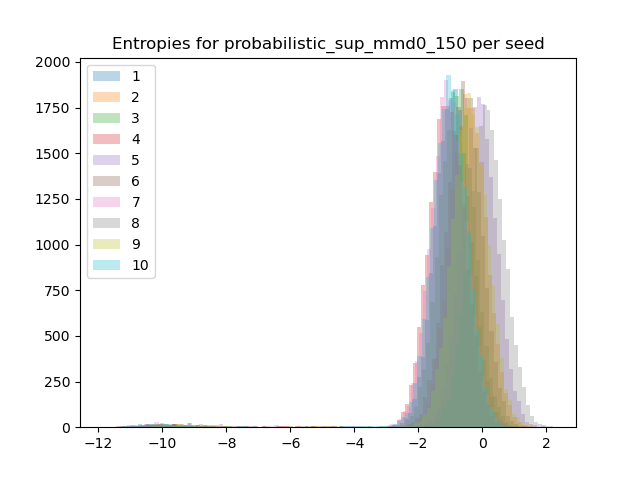
\includegraphics[width=0.6\textwidth]{images/method/probabilistic_aligned/openimages/probabilistic_sup_mmd0_150_entropies.png}
    \caption{
        Histogram of entropies for aligned Open Images embeddings, run without MMD. The plot is very faintly bimodal and there is more variability in it over runs with different random seeds than the entropy plot for the independently learned embeddings. 
    }
\end{figure}

\begin{figure}[H]

    \centering
    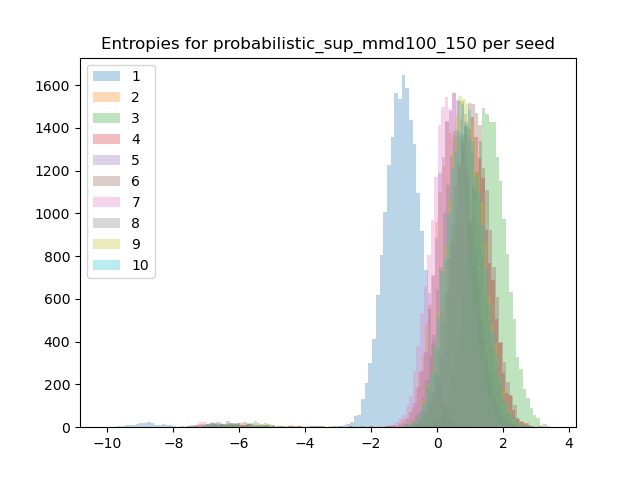
\includegraphics[width=0.6\textwidth]{images/method/probabilistic_aligned/openimages/probabilistic_sup_mmd100_150_entropies.png}
    \caption{
        Histogram of entropies for aligned Open Images embeddings, run with MMD. There is even more variability in the distributions between runs with different random seeds. 
    }
\end{figure}

\begin{figure}[H]
    \centering
    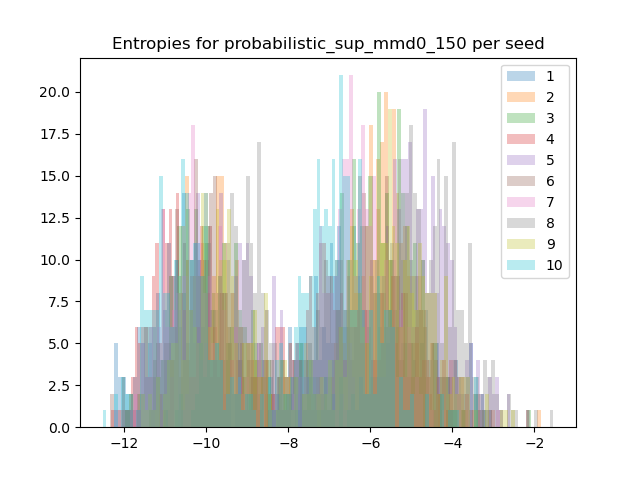
\includegraphics[width=0.6\textwidth]{images/method/probabilistic_aligned/audioset/probabilistic_sup_mmd0_150_entropies.png}
    \caption{
        Histogram of entropies for aligned AudioSet embeddings, run without MMD. The same pattern of bimodality plus greater variability is observed as in Open Images. 
    }
\end{figure}

\begin{figure}[H]

    \centering
    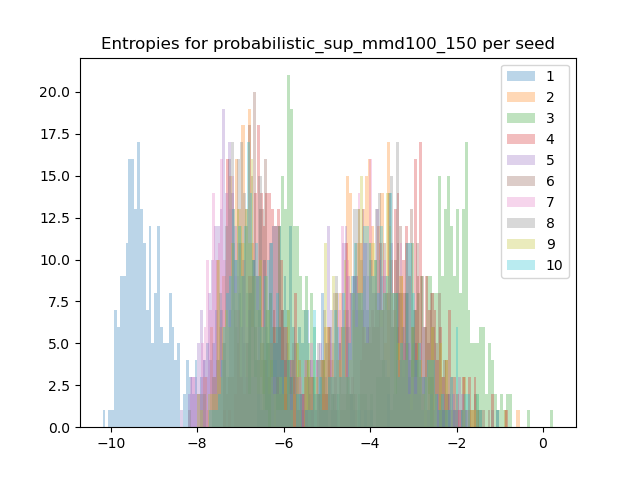
\includegraphics[width=0.6\textwidth]{images/method/probabilistic_aligned/audioset/probabilistic_sup_mmd100_150_entropies.png}
    \caption{
        Histogram of entropies for aligned AudioSet embeddings, run with MMD. Again, the same pattern of even greater variability between runs with different random seeds, is observed as in Open Images. 
    }
\end{figure}

\subsubsection{Alignment accuracy and embedding quality}

\begin{itemize}
    \item Using only distance (supervised) loss had a lower degree of accuracy - 94-95\% 
    \item Adding MMD gave a higher degree of accuracy - 96-97\%
\end{itemize}

High alignment accuracy between embeddings in both domains does not necessarily mean the embeddings are good. The following figure is a t-SNE plot of aligned embeddings (reduced to 2 dimensions) of very high accuracy (97\%), meaning that the embeddings in Open Images and AudioSet are well aligned. However, the actual embeddings did not form good clusters; concepts that were related semantically tended not to be close in embedding space. 

The following figure shows the results of running the alignment algorithm without scaling the GloVe loss:

\begin{figure}[H]
\label{fig:dysfunctional_clusters}
    \centering
    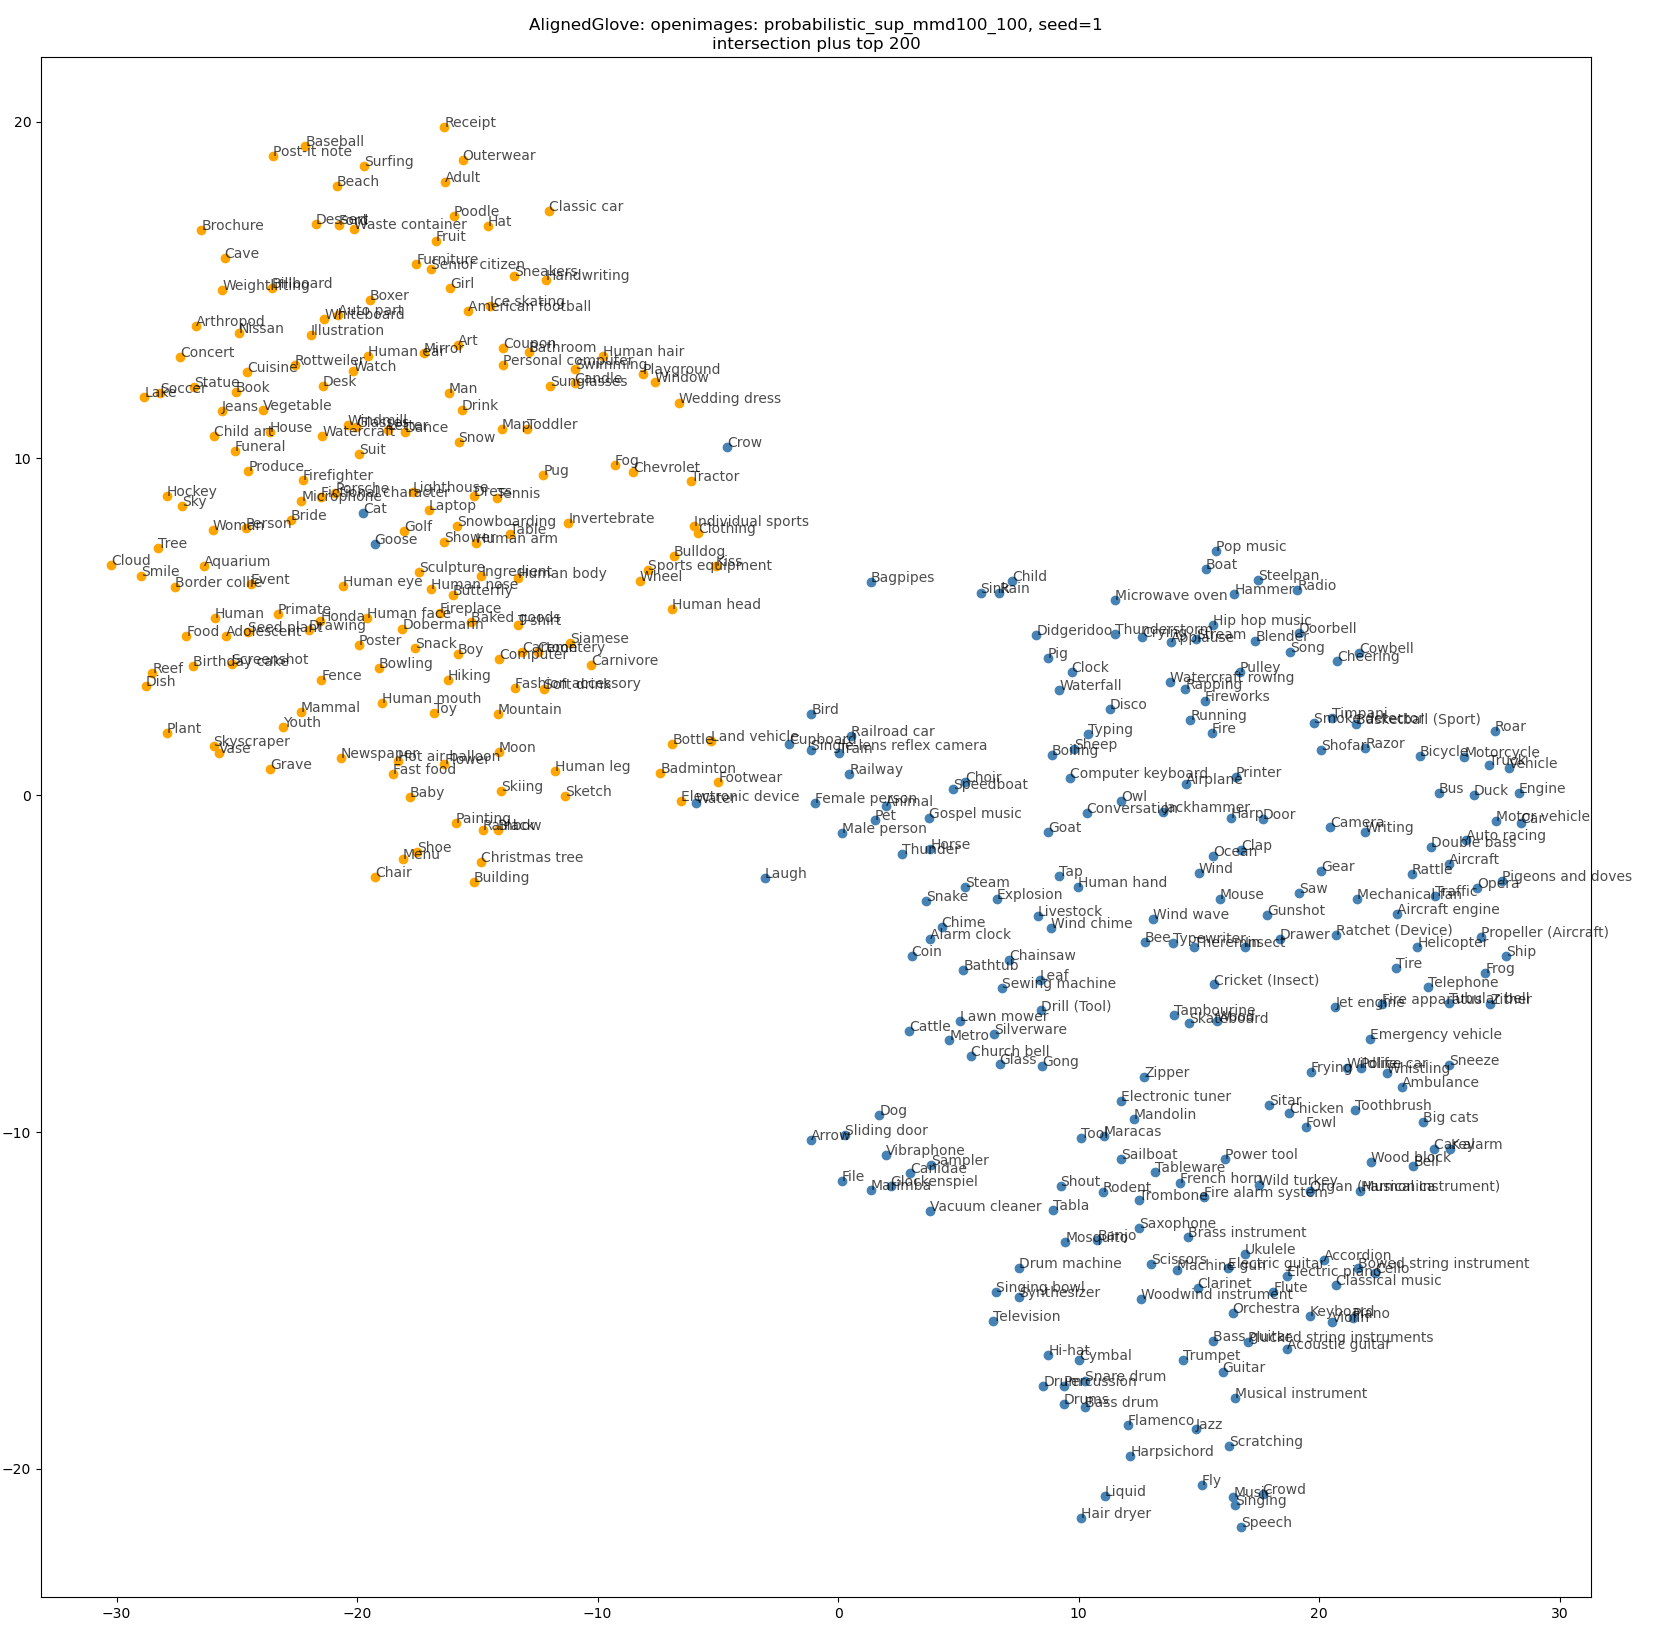
\includegraphics[width=0.95\textwidth]{images/method/probabilistic_aligned/dysfunctional_clusters.png}
    \caption{
        The alignment accuracy for this set of embeddings is greater than 97\%. The blue marks denote concepts that are in the intersection of concepts (present in both Open Images and AudioSet). The orange marks denote concepts that are in the 200 most frequent concepts occurring in Open Images. It is immediately visible that the algorithm has clustered concepts in the intersection degenerately; concepts that are in the intersection are more likely to be close to other concepts in the intersection rather than concepts that are semantically close
    }
\end{figure}

Hence, alignment accuracy is insufficient and we need another metric. To evaluate the quality of the resulting aligned embeddings, we could compare how good they are relative to independently learned embeddings. If our alignment algorithm is good, we should expect that the aligned embeddings are of higher quality than the independently learned embeddings. 

A plausible measure of embedding quality would be to compare the similarity of concept pairs as calculated from embeddings, with the similarity of concept pairs as evaluated by humans. In order to do this, we need to find human-curated datasets.

One such dataset is the MTURK-771 dataset, created by the authors of \cite{mturk771}, a study of learning the relatedness of word pairs. This study also uses the technique of measuring the goodness of their relatedness-learning algorithm by comparing the Spearman correlation of its predictions with the human judgements. The MTURK-771 dataset comprises 771 pairs of words with human-rated similarity scores, collected using the Amazon Mechanical Turk online tool. Unfortunately, the intersection of the 771 word pairs with our Open Images and AudioSet concepts was not large - 200+ \todo[inline]{GET EXACT NUMBER} for Open Images and only 3 for AudioSet. Therefore, this dataset is not sufficient for comparison. 

The WordNet \cite{WordNet} lexical database contains English nouns, verbs and adjectives grouped according to synonymy (semantic similarity) and hyponymy (hierarchy). Words in WordNet are represented by ``synsets", each of which denotes a particular sense of the word. Therefore, one word may have several synsets within WordNet. The relationships between word senses were encoded from various corpora and thesauri \todo[inline]{this seems wrong but thesauruses sounds stupid???}, which themselves were human-curated, therefore we take the lexical and semantic information contained within WordNet as an appropriate representation of human judgement. The WordNet database can be accessed directly from the \texttt{nltk} Python package. 

Furthermore, there is a large overlap between pairs of words found in WordNet and pairs of concepts from our dataset.  Out of 128005400 nonzero pairs occurring in Open Images, 27052350 are also present in WordNet. Out of 42002 nonzero pairs in AudioSet, 19208 are also present in WordNet. 

We adopt the same method used by \cite{mturk771} of comparing the Spearman correlation of the similarity of our embedding concept pairs with the similarity of the human-measured dataset to evaluate the quality of aligned embeddings compared to independently learned embeddings. The Spearman correlation is used because we wish to evaluate whether there is a monotonic relationship, and the similarity measures will be on different scales. The dot product is used as the similarity measure as it is an input into the GloVe algorithm that generates the `embeddings.

The similarity of two concepts with indexes $i$ and $j$ in embedding space is therefore measured as

\begin{equation}
s_{ij} &= \vece_i \cdot \vece_j
\end{equation}

where $\vece$ represents the embedding. 

WordNet has various available similarity measures between synsets that can be computed directly from the Python library. We choose the Leacock-Chodorow (LCH) similarity measure (https://citeseerx.ist.psu.edu/viewdoc/download?doi=10.1.1.14.1677&rep=rep1&type=pdf), which takes the shortest path between the two synsets, scaled by the maximum depth of the taxonomy \todo[inline]{DEFINE THIS}. Intuitively, if the two synsets are very similar, there will be a short path between them, and they will have a common ancestor that is not many levels up in the hierarchy. 

As a single word or phrase may map to several synsets, and we have no sense information in our Open Images / AudioSet concept names to disambiguate, we have to use a heuristic algorithm for choosing a synset in the cases where there is more than one:

\begin{itemize}
    \item Check every pair in the domain (Open Images or AudioSet) that has nonzero co-occurrence
    \item Convert each word in the pair to lowercase with spaces replaced with underscores, as this is the WordNet naming scheme.
    \item Check if both converted words have synsets represented in WordNet. If either does not have a synset in WordNet, ignore the pair.
    \item For each combination of the first 2 synsets for each word (up to 4 pairs in total), compute the LCH similarity \todo{CITE} if both elements in the pair have the same part of speech. If they do not have the same parts of speech, ignore the pair. \footnote{WordNet similarity is not defined for synsets which do not have the same parts of speech. } This is to handle pairs like ``mandarin orange" and ``orange"; ``mandarin orange" has two synsets, the first of which refers to the mandarin orange tree, and the second of which refers to the fruit. Therefore the second ``mandarin orange" synset matches the first ``orange" synset more closely. 
    \item The WordNet similarity for the pair is taken to be the largest such value. Therefore this algorithm will be biased high; thus if we observe a strong effect in spite of this high bias, it is a stronger result. 
\end{itemize}

If the Spearman correlation between the aligned embedding pair similarity and WordNet pair similarity is higher than the Spearman correlation between the independently learned embedding pair similarity and WordNet pair similarity, it indicates that the aligned embedding pairs are in aggregate more like human judgement of similarity than the independent embedding pairs. Since our goal is to obtain embeddings that are more similar to human judgement, this would translate to the aligned embeddings being of higher quality, by this metric. We can generalise this to other model variants, for example aligning with or without the MMD loss, to evaluate the effect of those model variants. 

\subsubsection{Open Images, Spearman correlation with WordNet similarity}

\begin{tabular}{lrrrrr}
\toprule
{} &  independent &   aligned &  aligned\_acc &  aligned\_mmd &  aligned\_mmd\_acc \\
\midrule
1    &     0.146461 &  0.206897 &     0.947826 &     0.207112 &         0.947826 \\
2    &     0.146638 &  0.190739 &     0.956522 &     0.204374 &         0.982609 \\
3    &     0.146598 &  0.220325 &     0.934783 &     0.224408 &         0.956522 \\
4    &     0.146336 &  0.211183 &     0.952174 &     0.207201 &         0.965217 \\
5    &     0.147186 &  0.199297 &     0.947826 &     0.202284 &         0.960870 \\
6    &     0.146104 &  0.217810 &     0.952174 &     0.218575 &         0.973913 \\
7    &     0.146059 &  0.205329 &     0.965217 &     0.219786 &         0.965217 \\
8    &     0.147155 &  0.190543 &     0.969565 &     0.194335 &         0.952174 \\
9    &     0.146923 &  0.196938 &     0.956522 &     0.212506 &         0.956522 \\
10   &     0.146870 &  0.202247 &     0.960870 &     0.211041 &         0.952174 \\
mean &     0.146633 &  0.204131 &     0.954348 &     0.210162 &         0.961304 \\
\bottomrule
\end{tabular}




\subsubsection{Open Images, differences of Spearman correlation between aligned model variant and WordNet and independent embeddings} with WordNet\\


\begin{tabular}{lrr}
\toprule
{} &   aligned &  aligned\_mmd \\
\midrule
1    &  0.060436 &     0.060651 \\
2    &  0.044100 &     0.057736 \\
3    &  0.073727 &     0.077810 \\
4    &  0.064847 &     0.060866 \\
5    &  0.052110 &     0.055098 \\
6    &  0.071706 &     0.072471 \\
7    &  0.059271 &     0.073727 \\
8    &  0.043389 &     0.047181 \\
9    &  0.050014 &     0.065583 \\
10   &  0.055377 &     0.064171 \\
mean &  0.057498 &     0.063529 \\
\bottomrule
\end{tabular}





\subsubsection{AudioSet, Spearman correlation with WordNet similarity}

\begin{tabular}{lrrrrr}
\toprule
{} &  independent &   aligned &  aligned\_acc &  aligned\_mmd &  aligned\_mmd\_acc \\
\midrule
1    &     0.152214 &  0.134991 &     0.947826 &     0.146133 &         0.965217 \\
2    &     0.150857 &  0.117635 &     0.969565 &     0.137159 &         0.982609 \\
3    &     0.145463 &  0.149323 &     0.956522 &     0.121679 &         0.978261 \\
4    &     0.155565 &  0.139078 &     0.956522 &     0.164043 &         0.956522 \\
5    &     0.157137 &  0.132362 &     0.943478 &     0.144181 &         0.969565 \\
6    &     0.152070 &  0.112995 &     0.973913 &     0.115492 &         0.969565 \\
7    &     0.149935 &  0.109444 &     0.947826 &     0.167198 &         0.973913 \\
8    &     0.154389 &  0.166478 &     0.960870 &     0.119457 &         0.952174 \\
9    &     0.157271 &  0.114488 &     0.960870 &     0.186357 &         0.978261 \\
10   &     0.155973 &  0.145066 &     0.965217 &     0.130960 &         0.978261 \\
mean &     0.153087 &  0.132186 &     0.958261 &     0.143266 &         0.970435 \\
\bottomrule
\end{tabular}


\subsubsection{AudioSet, differences of Spearman correlation between aligned model variant and WordNet and independent embeddings with WordNet}

\begin{tabular}{lrr}
\toprule
{} &   aligned &  aligned\_mmd \\
\midrule
1    & -0.017223 &    -0.006081 \\
2    & -0.033222 &    -0.013698 \\
3    &  0.003861 &    -0.023783 \\
4    & -0.016487 &     0.008478 \\
5    & -0.024775 &    -0.012956 \\
6    & -0.039075 &    -0.036577 \\
7    & -0.040491 &     0.017263 \\
8    &  0.012089 &    -0.034933 \\
9    & -0.042784 &     0.029085 \\
10   & -0.010906 &    -0.025013 \\
mean & -0.020901 &    -0.009821 \\
\bottomrule
\end{tabular}


\subsubsection{Discussion}
\begin{itemize}
    \item Open Images:
    \begin{itemize}
        \item For Open Images, using the WordNet comparison metric, it appears that the aligned embeddings are more correlated with human similarity judgement than the independently learned embeddings. 
        \item MMD appears to give a further increase in embedding quality, as measured by the difference of the means of Spearman correlation between model variants and independent embeddings.
        \item In addition, MMD appears to increase accuracy. 
    \end{itemize}
    \item AudioSet:
    \begin{itemize}
        \item For AudioSet, the trend is in the other direction: It appears that the aligned embeddings are on average less correlated with human similarity judgement than the independently learned embeddings, as measured by comparing with WordNet. However MMD still has a positive effect on both correlation and accuracy. 
    \end{itemize}
    \item Using MMD as a loss function has the effect of forcing $f(x)$ and $y$ to have the same distribution, and  $g(y)$ and $x$ to have the same distribution. Therefore it is reasonable that it should have a positive effect on alignment accuracy. 
    \item However if MMD is high relative to glove loss, there is more pressure for alignment but less pressure for good embeddings which can result in dysfunctional embeddings where all the concepts in the intersection are clustered together as shown in figure \ref{fig:dysfunctional_cluster}
\end{itemize}
